\pagebreak
\chapter{Memoria virtuale}\label{virtual memory}
In questo capitolo cerchiamo di capire com un sistema operativo gestisce la memoria attraverso le tecniche che abbiamo visto nel capitolo precedente (\ref{main memory}). Ci occuperemo prima di tutto del concetto di \textit{demand paging} e alcune tecniche di ottimizzazione come il \textit{copy-on-write}. In secondo luogo passeremo a discutere di tutti gli algoritmi di rimpiazzo delle pagine (\textit{page replacement}) in memoria. Discuteremo infine il fenomeno del \textit{thrashing} e di alcune soluzioni che adottano i moderni sistemi operativi.

% 
\section{Introduzione}
Sappiamo che il codice, al fine di essere eseguito, deve essere presente nella memoria. Quando parliamo di memoria virtuale, parliamo infatti della separazione tra indirizzo logico e fisico. Fino ad ora abbiamo discusso di processi che, anche se divisi in pagine o in segmenti, venivano comunque caricati tutti in memoria. Da adesso introduciamo la possibilità di poter eseguire un processo anche se le sue pagine non sono tutte in memoria, anzi, possono risiedere sul file system (\ref{file system}) o sul \textit{backing store}. Infatti quando un processo è eseguito, non è necessario che l'intero codice del programma sia in memoria, è sufficiente solo un sottoinsieme. Osservando infatti la figura \ref{fig:virtual_memory}, possiamo notare che le pagine nella memoria virtuale non sono tutte presenti nella memoria fisica, bensì alcune risiedono nei backing store.
\begin{figure}[h]
    \centering
    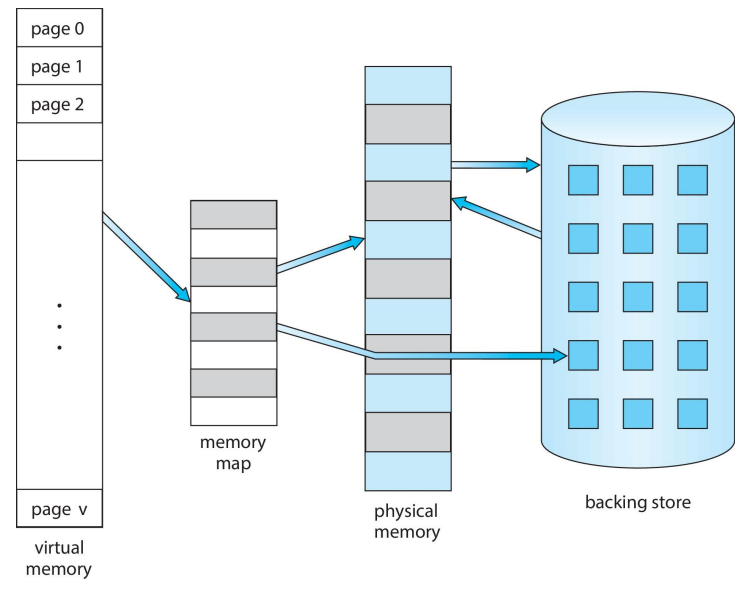
\includegraphics[width = .6\textwidth]{../res/imgs/virtual memory/virtual_memory.png}
    \caption{Alcune pagine del processo sono in memoria, altre sono sul disco.}
    \label{fig:virtual_memory}
\end{figure}

% 
\subsection{Spazio degli indirizzi virtuali}
Quello che nel capitolo precedente abbiamo definito come lo spazio degli indirizzo logici in realtà si chiama più propriamente spazio di indirizzi virtuali. Questo è lo spazio degli indirizzi che il programma vede: per ogni programma quindi questo spazio parte dell'indirizzo zero e consiste in un insieme di indirizzi continui. L'implementazione di questo spazio virtuale può essere effettuata attraverso delle tecniche di paginazione o segmentazione chiamate come \textit{demand paging} e \textit{demand segmentation}. 

Il fatto di riuscire ad implementare uno spazio di indirizzi virtuali contigui ci permette di implementare delle strutture che dal punto di vista virtuale sono quelle viste dal processo (come la figura \ref{fig:memory_layout} nel capitolo \ref{processes}).

% 
\subsection{Memoria condivisa}
Tramite la dinamicità fornita dalla memoria virtuale è possibile mappare delle zone in memoria condivise e quindi avere dei riferimenti in processi diversi alla stessa zona in memoria (\ref{fig:shared_pages}). 
\begin{figure}[h]
    \centering
    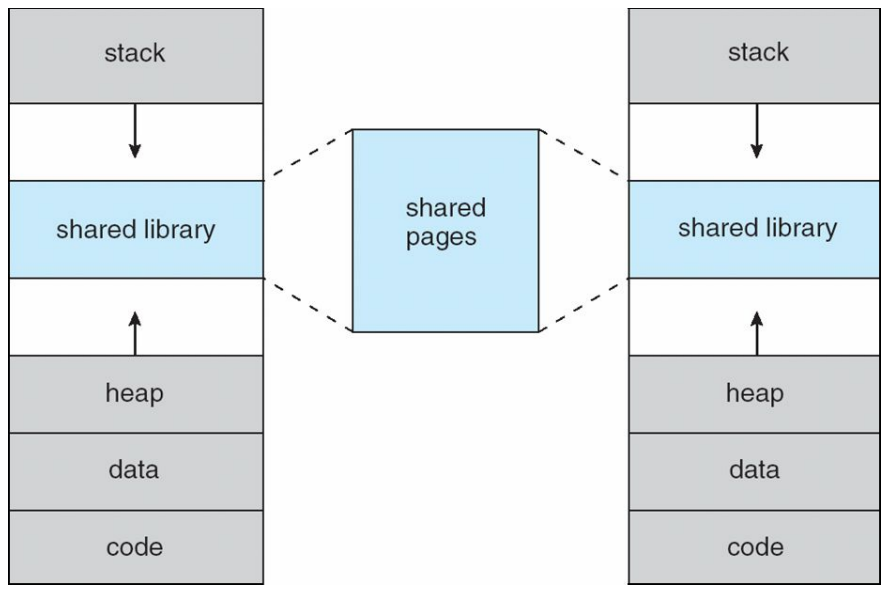
\includegraphics[width = .4\textwidth]{../res/imgs/virtual memory/shared_pages.png}
    \caption{La memoria virtuale fornisce la possibilità di condividere delle librerie.}
    \label{fig:shared_pages}
\end{figure}
In queste zone di memoria possono essere condivise delle librerie, come nel caso delle \texttt{dll}, viste nel paragrafo \ref{dynamic loading and linking}, oppure utilizzare questa zona per della comunicazione tra processo, ovvero la IPC, \textit{Inter Process Communication} (\ref{IPC}).

% 
\section{Demand Paging}
Al fine di essere in grado di trasformare tutti i \textit{virtual address space} in indirizzi fisici caricando solo le pagine che vengono utilizzate e non tutte le pagine del processo si utilizza la tecnica del \textbf{demand paging}, illustrato in figura \ref{fig:demand_paging}. Ciò significa che se abbiamo dei processi A e B che richiedono delle particolari pagine (contenenti codice o dati), si andranno a caricare quelle pagine su domanda dal \textit{secondary storage} (come l'hard disk) alla memoria principale.
\begin{figure}[h]
    \centering
    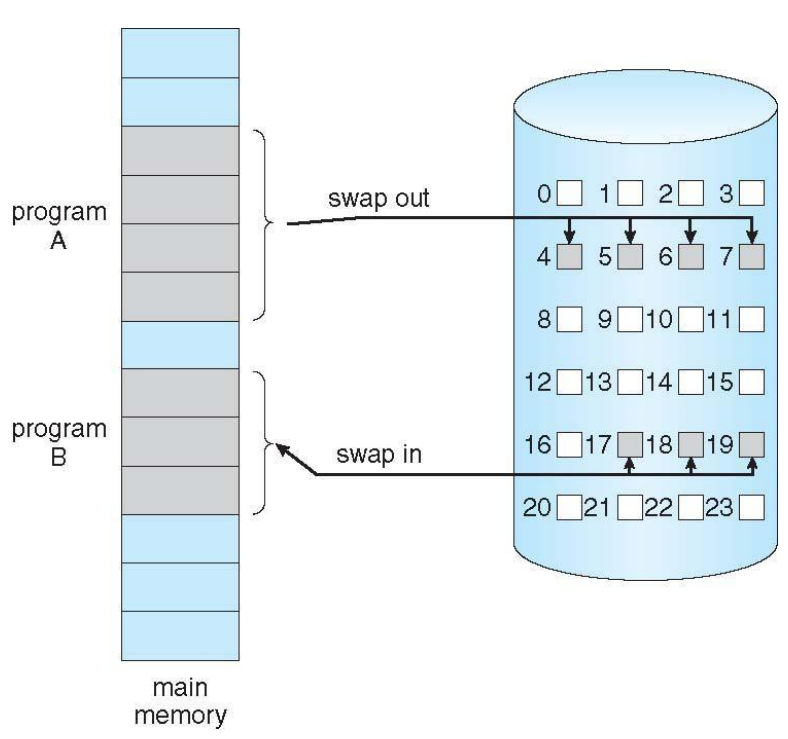
\includegraphics[width = .55\textwidth]{../res/imgs/virtual memory/demand_paging.png}
    \caption{Illustrazione del funzionamento del demand paging nel caso di due processi, A e B.}
    \label{fig:demand_paging}
\end{figure}
Dovremo quindi essere in grado di gestire questa richiesta per caricare dalla memoria secondarie le pagine oppure per scaricare le pagine dalla memoria principale, ovvero la memoria RAM. Al fine di riuscirci, ci appoggeremo a dei supporti hardware come il \textbf{bit di reference} che indica se la pagina di cui abbiamo bisogno è in memoria o sullo storage secondario. Nel caso in cui la pagina si trova già in memoria si dice infatti che la pagina è \textbf{memory resident}, ovvero che è immediatamente disponibile.

%
\subsection{Page fault}\label{page fault}
Per garantire che in memoria ci sia sempre il set di pagine richiesto si avrà bisgno del supporto hardware, in particolare si fa riferimento alle funzionalità della MMU. In particolare, questa fornisce la possibilità di settare il \textit{valid/invalid bit} - nella tabella delle pagine - il quale indica se la pagina che andiamo a richiedere è già presente in memoria o meno. Se la pagina non è in memoria si genera un interrupt chiamato \textbf{page fault} che deve essere ovviamente gestito dal sistema operativo.

Osserviamo la figura \ref{fig:page_fault}. Abbiamo a che fare con un processo che richiede 8 pagine che però non sono presenti tutte in memoria: dalla \textit{page table} possiamo notare che la pagina A è in memoria e si trova nel frame 4, la pagina C è associata al frame 6 e infine la pagina F è associata al frame 9. 
\begin{figure}[h]
    \centering
    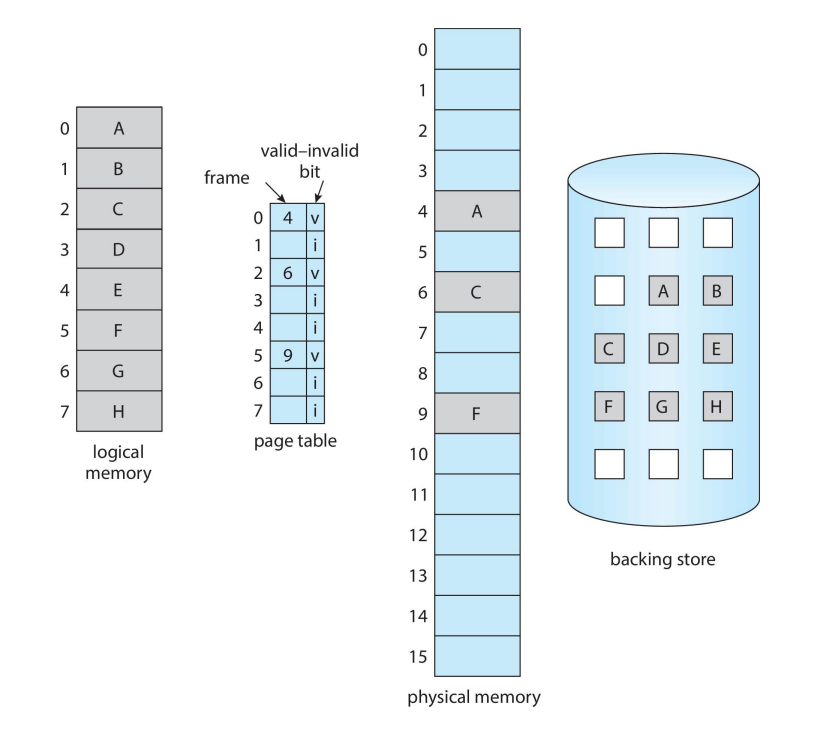
\includegraphics[width = .50\textwidth]{../res/imgs/virtual memory/page_fault.png}
    \caption{Generazione di un page fault.}
    \label{fig:page_fault}
\end{figure}
Tutte le altre pagine non sono presenti in memoria e quindi il loro \textit{invalid bit} è impostato a "v". Per quanto riguarda le altre pagine invece si verificano dei \textit{page fault} dato che non si trovano in memoria ma solo nel \textit{backing store}: possiamo infatti notare che l'\textit{invalid bit} di queste pagine è settato a "i". 

Come si comporta il sistema operativo adesso? Basandoci sull'illustrazione \ref{fig:page_fault_handling}, possiamo osservare che ci sono 6 steps da compiere. 
\begin{figure}[h]
    \centering
    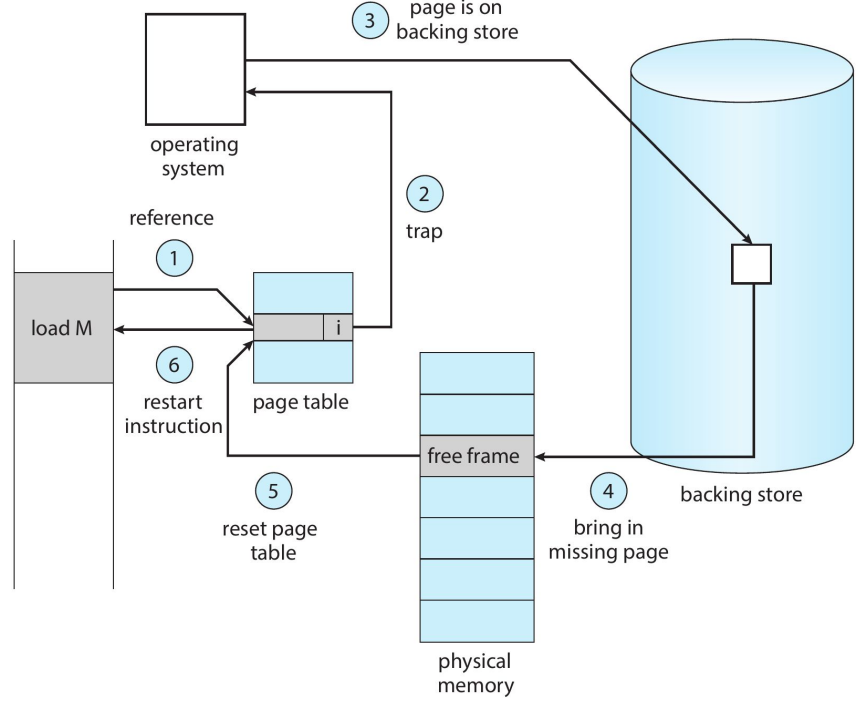
\includegraphics[width = .55 \textwidth]{../res/imgs/virtual memory/page_fault_handling.png}
    \caption{Gli steps necessari per prelevare la pagina dallo storage secondario}
    \label{fig:page_fault_handling}
\end{figure}
Dopo aver richiesto la pagina (punto 1) e, mediante la page table, aver constatato che non è presente in memoria (punto 2), il sistema operativo cattura il page fault e va a cercare il frame sulla memoria secondaria (punto 3). Assumendo che ci siano sempre degli spazi liberi in memoria, il sistema operativo ne sceglie uno e inserisce il frame che ha trovato sul \textit{backing store} (punto 4). A questo punto aggiorna l'\textit{invalid bit} sulla \textit{page table} e specifica in quale frame si trova la pagina virtuale (punto 5). Infine l'istruzione viene fatta ripartire (punto 6): in questo modo l'istruzione può essere eseguita e il processo può continuare.

%
\subsection{Pure demand paging}
Appena iniziamo l'esecuzione di un processo, questo deve ancora essere caricato in memoria. Ebbene, il demand paging puro consiste nel caricare solo le pagine del processo che vengono richieste. In altre parole il processo viene caricato in memoria frammento dopo frammento. Questo, per quanto istintivo possa sembrare, è in realtà estremamente \textbf{inefficiente}: significherebbe aumentare generare un numero elevatissimo di \textit{page fault} e di conseguenza il sistema operativo dovrebbe passare per il \textit{backing store} molte volte. Fortunatamente però i processi godono di una proprietà chiamata \textbf{locality of reference}: questo significa che la maggior parte del codice e dei dati di un processo è raggruppata tutta assieme e non sono sparpagliati nella memoria.

Un approccio sicuramente più efficiente è quello di cercare di caricare il maggior numero di pagine possibili in memoria al fine di minimizzare il numero di page fault e quindi di accessi alla memoria secondaria.

% 
\subsubsection*{Gestione della memoria libera}
Fino ad ora abbiamo assunto che ci siano sempre dei frame liberi in memoria ma naturalmente non è così (vedi paragrafo \ref{page replacement}). Il sistema operativo possiede quindi una lista dei frame che sono liberi, la cosiddetta \textbf{free-frame list}, che viene utilizzata per identificata dove poter inserire la nuova pagina. Nel caso non ci siano elementi liberi è necessario liberare dello spazio in memoria attraverso gli algoritmi di rimpiazzo (paragrafo \ref{page replacement}).

Nel momento in cui dei frame vengono liberati tramite questi algoritmi va ad azzerare il contenuto utilizzato precedentemente, in modo tale da garantire che il nuovo processo non vada a leggere dati che appartengono al vecchio processo. Questa tecnica è chiamata \textbf{zero-fill-on-demand}.

% 
\subsection{Performance e ottimizzazione}
Come abbiamo visto, nel momento in cui viene catturato un page fault il tempo perso a sostituire la pagina desiderata è notevole. Ci sono molte cause che portano le tempistiche ad essere così elevate però, generalmente le principali sono le tre seguenti:
\vspace{-5px}
\begin{enumerate}
\setlength{\itemsep}{-.25 em}
    \item La \textit{routne} che gestisce il page fault;
    \item Il tempo per leggere la pagina dal disco;
    \item Il tempo necessario per far ripartire il processo (ricaricare i dati e i registri nel momenti in cui la pagina è in memoria).
\end{enumerate}
Per valutare le performance del demand paging ci si basa su una variabile chiamata \textbf{page fault rate}, che è la frequenza con cui un page fault avviene. Quando questa vale 0, non si verificano mai questi interrupt, quando è 1 si verificano ad ogni nuova esecuzione che viene eseguita. Ovviamente, il nostro obiettivo è quello di minimizzare il più possibile questo fattore. Questo valore lo utilizziamo per calcolare l'\textbf{EAT} (\textit{Effective Access Time}), ovvero il tempo di accesso reale, effettivo. Sia $p$ il \textit{page fault rate}, per calcolare l'EAT si utilizza la seguente formula:
\begin{gather*}
    (1-p)\cdot\text{Memory Access Time} + \\  p\cdot(\text{Page fault Overhead} + \text{Swap Page Out} + \text{Swap Page In})
\end{gather*}
Al fine di riuscire a diminuire l'EAT si può cercare di ottimizzare alcuni aspetti. Si può cercare di diminuire il tempo di \textit{swap-out} e di \textit{swap-in} dei frame nella memoria oppure si può cercare di copiare l'intero processo sullo swap space. Si possono sfruttare anche altre proprietà dei processi: se le pagine che abbiamo in memoria che devono essere sostituite non sono state modificate è sufficiente eliminare le pagine al posto di andarle a salvare sul disco (tanto sono uguali). 

Infine, una tecnica molto importante ed ingegnosa è quella del \textbf{Copy-On-Write} (figura \ref{fig:copy_on_write}) dove, nel momento in cui un processo padre viene \textit{forkato} (vedi \ref{creazione di un processo}), il processo figlio condivide le stesse pagine del padre: è molto più efficiente che copiare le stesse pagine due volte in memoria. Le pagine continuano ad essere condivise fino a che tali pagine non devono essere modificate: ecco perché si chiama in questo modo, una pagina viene copiata solo nel momento in cui si deve scrivere su di essa. 
\begin{figure}[h]
    \centering
    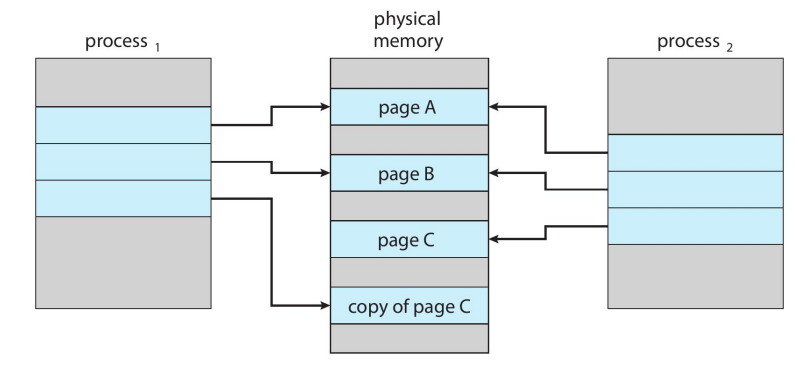
\includegraphics[width = .6\textwidth]{../res/imgs/virtual memory/copy_on_write.png}
    \caption{Dato che P1 deve scrivere sulla pagina C, questa viene copiata.}
    \label{fig:copy_on_write}
\end{figure}

% 
\subsection{Prepaging}
Contropposto al \textit{pure demand paging}, dove, dopo aver caricato il processo all'inizio, si caricano le pagine che necessita attraverso i page fault. Ovviamente, c'è anche la possibilità di non caricare solamente una pagina del processo, bensì caricare un insieme di pagine al fine di diminuire la frequenza di page fault e quindi risparmiare più tempo 



% 
\section{Page replacement}\label{page replacement}
Fino ad ora abbiamo dato per scontato che ci fosse sempre dello spazio libero in memoria. Spesso invece non è così e il sistema operativo si trova nella condizione di dover rimuovere una pagina dalla memoria per sostituirla con quella che è stata appena richiesta. Come scegliere la pagina da scartare? È proprio questo il compito di un \textbf{algoritmo di rimpiazzo}. Attraverso i \textit{replacemnt algorithms} ben studiati è quindi possibile avere una grande memoria virtuale in una memoria fisica di dimensioni ridotte.

Nella pratica le operazione generali di un algoritmo di rimpiazzo sono (vedi anche figura \ref{fig:replacement_algorithm}:
\vspace{-5px}
\begin{enumerate}
\setlength{\itemsep}{-.25 em}
    \item Selezionare un frame vittima dalla memoria e portarlo nel \textit{backing store} (\textit{swap out});
    \item Cambiare il bit nella page table da \textit{valid} a \textit{invalid};
    \item Copiare la nuova pagina dallo storage secondario alla memoria \textit{swap-in}); 
    \item Aggiornare l'invalid bit nella page table a valid.
\end{enumerate}
Osserviamo anche che in questi casi è aggiunto un altro bit, chiamato \textbf{dirty bit} che segnala se una pagina in memoria è stata modificata o meno. Di conseguenza se la pagina non è stata modificata viene rimossa, altrimenti deve essere copiata nella memoria secondaria. 
\begin{figure}[h]
    \centering
    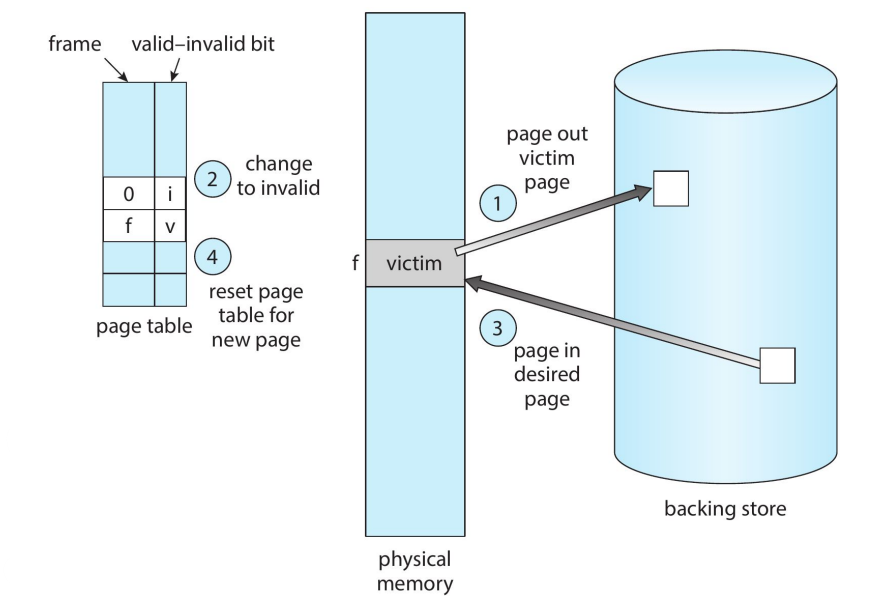
\includegraphics[width = .65\textwidth]{../res/imgs/virtual memory/replacement_algorithm.png}
    \caption{Funzionamento generico di un algoritmo di rimpiazzo.}
    \label{fig:replacement_algorithm}
\end{figure}

Ricordiamo che un algoritmo di \textit{page replacement} deve tenere conto di diversi aspetti. Innanzitutto bisogna capire quanti e quali frame devono essere assegnati per ciascun processo? È meglio avere una distribuzione equa oppure proporzionato all'importanza o alla priorità che hanno? In secondo luogo il compito di un algoritmo di rimpiazzo rimane quello di \textbf{ridurre} il \textbf{page fault} rate.

% 
\subsection{FIFO}
Il primo algoritmo che vediamo, come per lo scheduling e per altre occasione, è un algoritmo simile ad una coda: \textit{First In First Out}. In altre parole la vittima che si sceglie è il frame che è stato inserito in memoria meno recentemente.

Prendiamo in considerazione la stringa \texttt{\small 7 0 1 2 0 3 0 4 2 3 0 3 3 2 1 2 0 1 7 0 1}, dove ogni numero rappresenta la pagina che si sta richiedendo. Supponiamo inoltre, per semplicità, che la nostra memoria sia in gradi di contenere solamente 3 frames. Simuliamo una le richieste e contiamo il numero di \textit{page fault} che si sono verificati durante le richieste.
\begin{figure}[h]
    \centering
    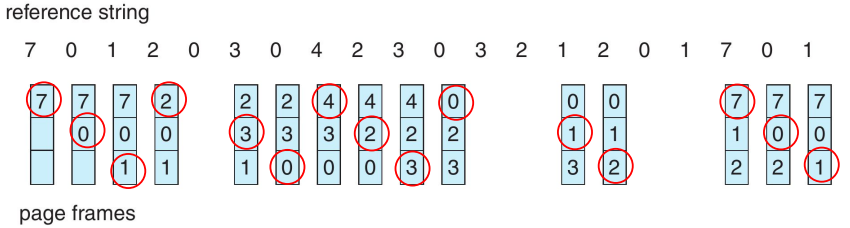
\includegraphics[width = .85\textwidth]{../res/imgs/virtual memory/FIFO_replacement.png}
    \caption{Comportamento dell'algoritmo di rimpiazzo FIFO.}
    \label{fig:FIFO_replacement}
\end{figure}
Commentiamo il comportamento di questo algoritmi basandoci sulla figura \ref{fig:FIFO_replacement}. Con le prime 3 pagine si verifica un \textit{page fault} in quanto la memoria da vuota deve riempirsi. Al quarto \textit{timestamp}\footnote{Con \textit{timestamp} si intende l'istante di tempo che stiamo esaminando.}, quando si ha bisogno della pagina \texttt{2}, questa non è presente in memoria, si verifica un page fault e si scambia pagina \texttt{2} con pagina \texttt{7} questo perché, tra le tre pagine presente, è stata la prima ad entrare e quindi è la più "vecchia". Osserviamo che al quinto \textit{timestamp}, si richiede la pagina \texttt{0} che però è già presente in memoria e quindi non si verifica alcun page fault. Proseguendo così per tutta la stringa possiamo notare che su 20 richieste si verificano 15 page fault.

Osserviamo un avvenimento curioso, chiamato \textbf{Belady's anomaly}. In modo contro-intuitivo, all'aggiungere di più frames si incrementa il numero di page fault anziché andarlo a diminuire. Dando un'occhiata alla figura \ref{fig:beladys} notiamo passando da 3 a 4 frames il numero di page fault cresce.
\begin{figure}[h]
    \centering
    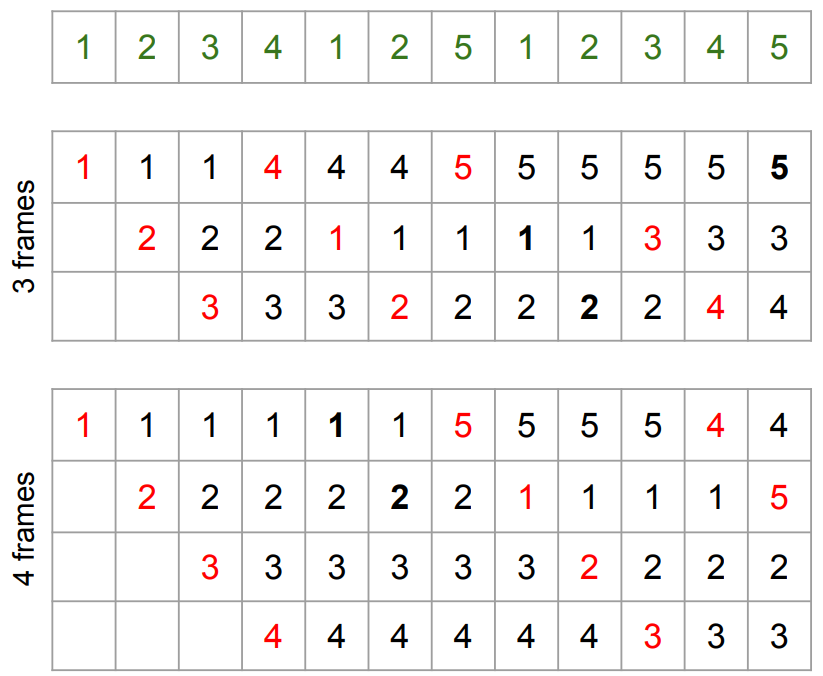
\includegraphics[width = .40\textwidth]{../res/imgs/virtual memory/belady1.png}
    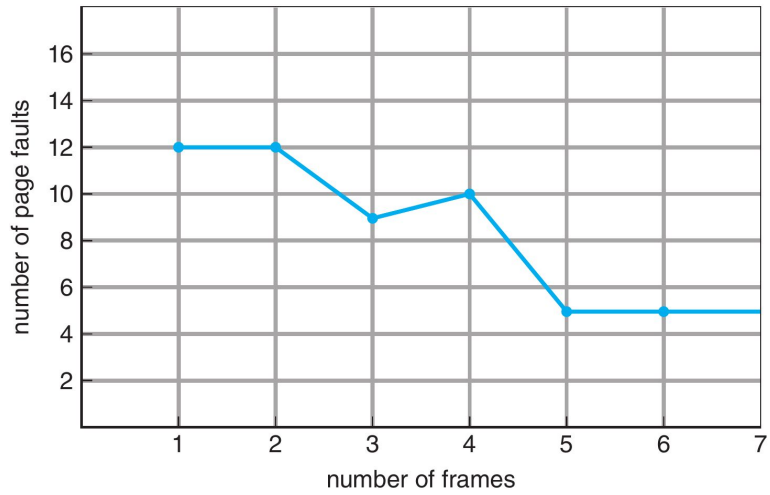
\includegraphics[width = .45\textwidth]{../res/imgs/virtual memory/belady2.png}
    \caption{Una piccola illustrazione dell'anomalia di Belady.}
    \label{fig:beladys}
\end{figure}

% 
\subsection{Algoritmo ottimale}
Il problema dell'algoritmo FIFO, oltre all'anomalia, è che nel momento in cui rimuoveva un frame dalla memoria non andava a domandarsi quanto questo frame è stato utilizzato e quindi senza tenere conto della storia dei frame. A livello teorico, un algoritmo ottimale rimuoverebbe il frame che verrà utilizzato il più tardi possibile nel futuro. Questo algoritmo è ovviamente utopico dato che conosce tutta la stringa. Nella realtà, ovviamente, non si è in grado di prevedere il futuro però si è in grado di fare delle buone stime.

Riprendiamo in considerazione la stringa \texttt{\small 7 0 1 2 0 3 0 4 2 3 0 3 3 2 1 2 0 1 7 0 1} e cerchiamo di capire come l'algoritmo ottimale rimpiazzi i frames all'interno della memoria (figura \ref{fig:optimal}). 
\begin{figure}[h]
    \centering
    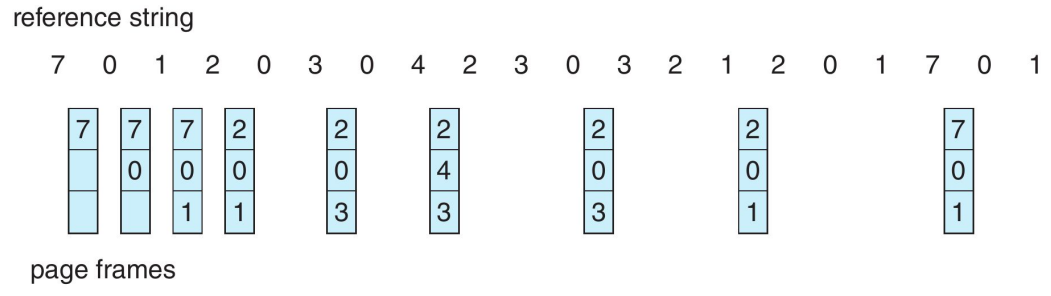
\includegraphics[width = .85\textwidth]{../res/imgs/virtual memory/optimal.png}
    \caption{Funzionamento teorica dell'algoritmo ottimale.}
    \label{fig:optimal}
\end{figure}
Dall'immagine notiamo che le prime tre richeste sono page fault dato che la memoria da vuota deve riempirsi. Al quarto \textit{timestamp} notiamo che anche in questo caso la pagina \texttt{7} viene rimossa perché è quella che viene utilizzata più tardi (verso la fine praticamente). Dopo di che, alla richiesta della pagina \texttt{0} non viene rimosso nulla perché verrà utilizzata nel futuro prossimo (più precisamente dopo due \textit{timestamp}). Proseguendo, quando viene richiesta la pagina \texttt{3} viene rimossa la pagina \texttt{1} dato che rispetto alla pagina \texttt{2} e \texttt{0} è quella che verrà utilizzata più tardi. Osserviamo che dalle 15 page fault dell'algoritmo FIFO riusciamo ad arrivare a 9. 

Dato che questo algoritmo non è realistico, questo serve come \textbf{caso limite} o caso ideale verso cui vogliamo che i nostri algoritmi vertano. È impossibile raggiungerci però ci si cerca di avvicinare il più possibile. Inoltre, sappiamo che un algoritmo, basandosi su questa stringa, non potrà avere meno di 9 page fault in quanto il limite è proprio stabilito dall'algoritmo ottimale.

%
\subsection{LRU}
Dato che non è possibile guardare nel futuro, questo algoritmo guarda il passato, la storia degli utilizzi delle pagine e fa una stima per cercare di capire quale saranno le prossime richieste. È proprio questo il funzionamento dell'algoritmo \textbf{LRU}, che sta per \textbf{\textit{Least Recently Used}}, ovvero il frame che è stato utilizzato meno tra quelli presenti nella memoria.

Prendiamo ancora una volta in considerazione la stringa \texttt{\small 7 0 1 2 0 3 0 4 2 3 0 3 3 2 1 2 0 1 7 0 1} e vediamo come questo algoritmo si comporta (figura \ref{fig:LRU}).
\begin{figure}[h]
    \centering
    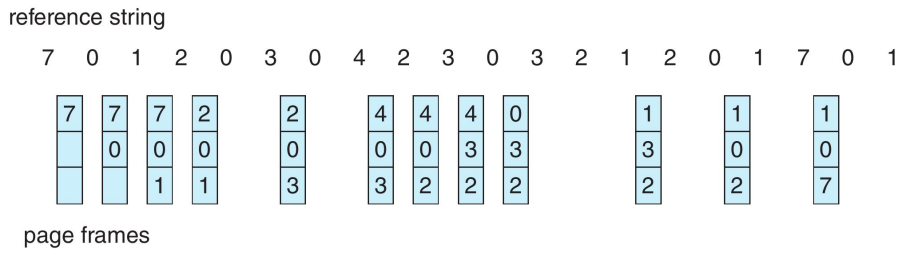
\includegraphics[width = .85\textwidth]{../res/imgs/virtual memory/LRU.png}
    \caption{Funzionamento dell'algoritmo LRU.}
    \label{fig:LRU}
\end{figure}
Come nei due casi precedenti, le prime quattro richieste sono page fault e la quinta no. Al sesto \textit{timestamp}, quando viene richiesta la pagina \texttt{3} l'algoritmo LRU sceglie di scartare il frame \texttt{1}, questo perché è stato quello utilizzato meno recentemente rispetto a \texttt{0} e \texttt{2}. A questo punto, la richiesta della pagina \texttt{0} non produce alcun page fault però la richiesta successiva, quella per la pagina \texttt{4} genera un interrupt che provoca la rimozione della pagina \texttt{2} in quanto è stata quella utilizzata meno rispetto alle pagine \texttt{0} e \texttt{3}. Procedendo in questa maniera scopriamo che il numero di page fault è 12, che sono 3 in meno rispetto all'algoritmo FIFO ma rimangono 3 in più rispetto all'algoritmo ottimale.

Com'è possibile implementare questo tipo di algoritmo? Non necessariamente abbiamo a che fare con dei \textit{timestamp} ma possiamo utilizzare un \textbf{contatore} mantenuto non dal sistema operativo bensì dall'hardware (come l'MMU), che incrementa il contatore ogni volta che c'è una reference a quella pagina. In questo modo, per scegliere quale pagina deve essere rimpiazzata, si controlla questo contatore e la pagina con il valore minore verrà scartata. Una seconda tecnica per implementare l'algoritmo LRU è attraverso uno \textbf{stack}: ogni volta che una pagina viene utilizzata viene impilata in cima allo stack e di conseguenza nel momento in cui si deve scegliere una pagina da rimpiazzare, quella che si troverà nel \textit{bottom} dello stack verrà scelta e scartata. Osserviamo che la seconda soluzione, a differenza del contatore, è una soluzione software piuttosto che hardware.

% 
\subsection{Second-chance (clock)}\label{second chance}
Questo algoritmo si basa sull'utilizzo di una \textbf{lista circolare} che contiene i riferimenti alle pagine che sono presenti in memoria e ogni qualvolta che di deve rimpiazzare una pagina in memoria con una nuova pagina appena richiesta si va a scorrere questa lista circolare. Ad ogni pagina caricata in memoria è associato un \texttt{bit}. Questo bit è impostato come segue:
\vspace{-4px}
\begin{itemize}
\setlength{\itemsep}{-1px}
    \item Il bit viene impostato a 1 ogni volta che la pagina in memoria è utilizzata dal processo;
    \item Il bit è impostato da 1 a 0 nel momento in cui la pagina presente non coincide con la pagina richiesta;
\end{itemize}
L'algoritmo quindi, nel momento in cui è necessario effettuare un rimpiazzo, scorre la lista fino a che non trova un bit a zero, e la pagina associata a quel bit viene rimossa. Tutti i bit a 1 che l'algoritmo ha incontrato prima di arrivare allo 0 sono impostati a zero. In questo modo, se la pagina non viene utilizzata a breve, al prossimo controllo dell'algoritmo questa verrà rimossa dalla memoria.

Facendo quindi riferimento alla figura \ref{fig:second_chance}, osserviamo che in memoria sono presenti 6 pagine in memoria. In particolare osserviamo che tutte le pagina tranne la numero 3 hanno il bit impostato ad 1: ciò significa che tutte le pagine, eccetto la terza, 
\begin{figure}[h]
    \centering
    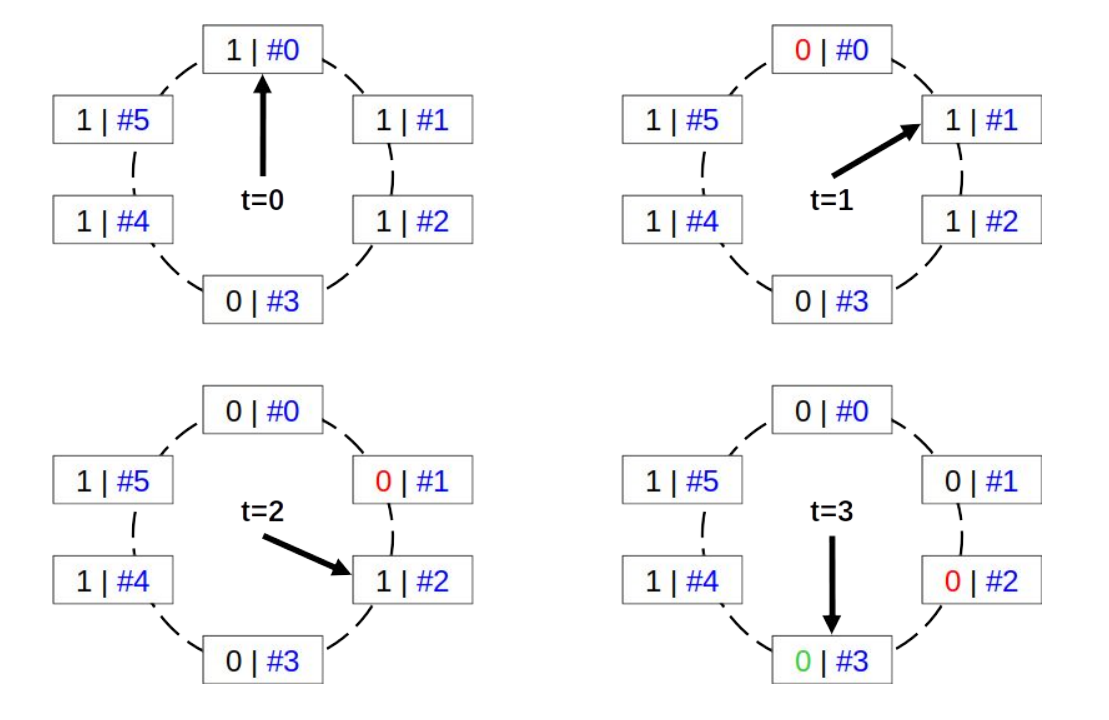
\includegraphics[width = .6\textwidth]{../res/imgs/virtual memory/second_chance.png}
    \caption{Il funzionamento del second-chance algorithm.}
    \label{fig:second_chance}
\end{figure}
Nel momento in cui è necessario rimpiazzare una pagina l'algoritmo parte dalla pagina 0 e comincia a scorrere. La pagina 0 è stata utilizzata poco prima perché il bit è a 1: di conseguenza l'algoritmo imposta il bit a zero e procede alla pagina seguente. Sia per la pagina 1 che per la pagina 2 l'algoritmo le lascia in memoria ma il bit diventa zero. Alla pagina numero 3 però il bit è già a zero, di conseguenza tale pagine verrà rimossa al fine di lasciare spazio a quelle nuova. 

È infine possibile migliorare questo approccio inserendo un secondo bit, chiaamto \textbf{modify bit} che indica se la pagina in memoria è stata modificata o meno. Si creano quindi quattro combinazioni possibili, e in base a queste l'algoritmo effettua delle azioni sulla pagina \texttt{(reference, modify)}:
\vspace{-4px}
\begin{itemize}
\setlength{\itemsep}{-1px}
    \item\texttt{(0,0)} indica che la pagina non è stata utilizzata recentemente e nemmeno modificata: è quindi la scelta migliore.
    \item\texttt{(0,1)} segnala che la pagina non è stata utilizzata di recente ma è stata modificata, di conseguenza, nel momento in cui la si rimpiazza, è necessario salvare le modifiche nel backing store.
    \item\texttt{(1,0)} indica che la pagina non è stata modificata ma è stata utilizzata di recente.
    \item\texttt{(1,1)} indica che la pagina è sia stata utilizzata di recente che modificata.
\end{itemize}

% 
\subsection{Algoritmo counting}
Oltre all'algoritmo LRU sono presenti anche altri tipi di approcci che si basano sul numero di utilizzi di una pagina. Le altre due opzioni che vediamo sono algoritmi che vanno a contare il numero di referenza fatte ad ogni singola pagina. A differenza quindi dell'algoritmo second-chance non si ha un bit che indica se la pagina è stata utilizzata di recente ma si ha un vero e proprio \textbf{contatore} che tiene traccia del numero di referenze alla determinata pagina in memoria.

Con questa informazione si possono quindi andare a rimuovere le pagine che sono state usate di meno, come nel caso dell'algoritmo \textbf{LFU} (\textit{Least Frequently Used}). Con questo approccio però può capitare che una pagina rimanga molto in memoria, anche se inutilizzata: poniamo il caso di una pagina nuova che entra in memoria e viene usata molto spesso. Questo significa che il contatore cresce subito e rimane alto. Anche se la pagina dopo molto tempo non è utilizzata, l'algoritmo non la rimuoverà mai dato che il contatore è molto alto. Si è quindi deciso di avere un check periodico dove si va a dimezzare il valore del contatore alle pagine che non sono utilizzate molto. In questo modo, prima o poi quella pagina in memoria se continua ad essere inutilizzata verrà rimossa appena il contatore diventa sufficientemente piccolo.

Un secondo approccio è quello opposto al LFU: stiamo infatti parlando del \textbf{MFU} (\textit{Most Frequently Used}), dove si va a rimuovere la pagina che ha il maggior numero di utilizzi.  

% 
\subsection{Ottimizzazione}
Oltre alle performance che si ottengono attraverso un algoritmo di page replacement si può cercare di ottimizzare l'algoritmo anche in altri momenti durante la procedura di rimpiazzo di una pagina. Per esempio è possibile implementare un insieme di \textbf{frame} sempre \textbf{liberi} (una sorta di buffer) al fine di allocare subito la pagina richiesta nel momento in cui si verifiche un page fault. Solo dopo aver soddisfatto la richiesta ci si preoccupa di rimuovere una pagina dalla memoria. In questo modo il processo viene immediatamente servito e non viene sprecato tempo prezioso al fine di scambiare le pagine dalla memoria la backing store. 

È possibile inoltre implementare una \textbf{lista delle pagine modificate}. Oltre al modify bit (\ref{second chance}), questa scelta è opportuna in quanto le pagine modificate contenute al suo interno verranno periodicamente salvate all'interno del backing store. In questo modo, una volta che ono state salvate la lista sarà vuota e il modify bit ritornerà a zero. 

%
\section{Allocazione dei frames}
Facciamo ora anche qualche considerazione riguardante il numero minimo e massimo di frames da allocare a ogni singolo processo. Ci sono diversi modi di allocare i frames per ciascun processo: poniamo di far partire 5 processi e che abbiamo a disposizione 100 frames. Possiamo scegliere di allocare i frames in maniera \textbf{uniforme}, dove ogni processo ha a disposizione 20 frames oppure, eventualmente, allocarne 15 per processo e tenere una \textit{pool} di 25 frames liberi. Altrimenti è possibile effettuare un'\textbf{allocazione proporzionale}: il numero di frames allocati per processo dipende dalla dimensione e dalla priorità di quest'ultimo. È infatti ragionevole che un processo di grandi dimensioni richiede un numero maggiore di frames rispetto ad un processo di dimensioni minori.

% 
\subsection{Allocazione globale e locale}
Quando andiamo a scegliere il frame da liberare al fine di fare spazio a nuove pagine, si possono scegliere due approcci.

Con l'approccio \textbf{globale} il frame da liberare viene scelto tra tutti i frame compresi in memoria, non importa a quale processo appartiene. In generale questo approccio è più performante rispetto al secondo e per questo è più utilizzato. 

Con l'approccio \textbf{locale} invece, per ogni processo viene definito un insieme di frames da dove è possibile andare a pescare. In questo caso invece le performance sono ridotte in quanto è possibile che ci siano frame liberi al di fuori dell'insieme scelto per il processo ma questi non potranno essere usati proprio perché non compresi nel frame. In questo caso però il vantaggio è che è più consistente nei tempi di risposta dato che sono presenti dei limiti ben definiti per allocare i frames. 

% 
\subsection{Richiesta delle pagine}
Al fine di riuscire ad implementare il \textit{global page replacement}, ovvero le classiche politiche di rimpiazzo, è quello di impostare dei limiti inferiori e superiori (\textit{thresholds}) al numero di frames liberi in memoria.
\begin{figure}[h]
    \centering
    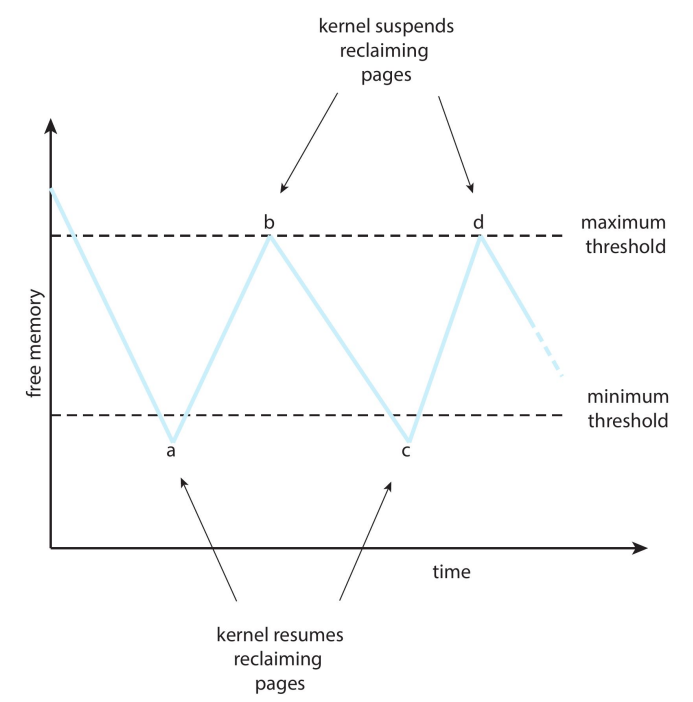
\includegraphics[width = .5\textwidth]{../res/imgs/virtual memory/reclaming_pages.png}
    \caption{Questa tecnica assicura la presenza di frames liberi in memoria al fine di soddisfare eventuali nuove richieste.} 
    \label{fig:reclaming_pages}
\end{figure}
Osservando la figura \ref{fig:reclaming_pages}, osserviamo che nel momento in cui il numero di frame disponibili scende sotto il limite inferiore, il sistema operativo esegue un algoritmo di page replacement al fine di liberare abbastanza frames da raggiungere il limite superiore. Nel caso in cui il sistema operativo non riesca a liberare la memoria, può scegliere di cambiare algoritmo di page replacement, magari scegliendone uno più \textit{strict}, oppure scegliere proprio di terminare qualche processo, potenzialmente quelli che consumano più memoria.

% 
\section{Thrashing}
Il thrashing è un aspetto importante, soprattutto perché diversi metodi, ormai superati, di gestione della memoria, non sono riusciti a gestire questo problema. La figura \ref{fig:thrashing} contiene uno schema dove viene mostrato l'utilizzo della CPU in relazione al numero di processi presenti in memoria.
\begin{figure}[h]
    \centering
    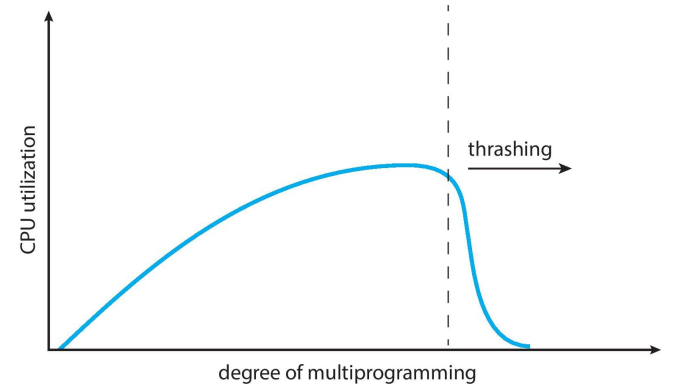
\includegraphics[width = .5\textwidth]{../res/imgs/virtual memory/thrashing.png}
    \caption{Il fenomeno del thrashing.}
    \label{fig:thrashing}
\end{figure}
Teoricamente l'obiettivo è quello di aumentare il numero di processi il più possibile al fine di aumentare l'utilizzo della CPU il più possibile. Notiamo in realtà che ad un certo punto l'utilizzo della CPU cala drasticamente. Questo generalmente capita quando il numero di processi in memoria è molto alto e quindi il numero di frames disponibili per processo diminuisce. Di conseguenza aumenta il numero di \textit{page fault} (\ref{page fault}) e quindi è necessario effettuare uno \textit{swapping} (\ref{swapping}). Lo swapping però non è effettuato dal processore, di conseguenza l'utilizzo della CPU diminuisce. Se l'utilizzo diminuisce allora il sistema operativo pensa che il processore sia pronto ad eseguire altri processi. Questi processi vengono quindi caricati in memoria, però non ci sono frames disponibili per loro e di conseguenza è necessario rimpiazzare delle pagine mediante uno swapping. Si entra quindi in un loop dove la CPU non viene utilizzata e tutti i processi non vengono eseguiti dato che si devono swappare tra di loro. 

% 
\subsection{Modello Working-set}
Al fine di cercare di evitare fenomeni di thrashing si può utilizzare una caratteristica che hanno i programmi, chiamata \textbf{locality model}. Questa caratteristica dei programma dice che tipicamente questi sono strutturati in modo tale che istruzioni e dati risiedi, sono raccolti, in zone di memoria \textbf{adiacenti}. Cerchiamo quindi di trovare un apporccio che sfrutti al meglio questo principio di località dei programmi.

Iniziamo definendo con $\Delta$ la finestra temporale dove avviene un certo numero di riferimenti alle pagine. Chiamiamo inoltre \textbf{WS} in \textit{working-set}, ovvero l'insieme di pagine che sono utilizzate all'interno di $\Delta$ (vedi figura \ref{fig:working-set}, dove la window è di 10 accessi).
\begin{figure}[h]
    \centering
    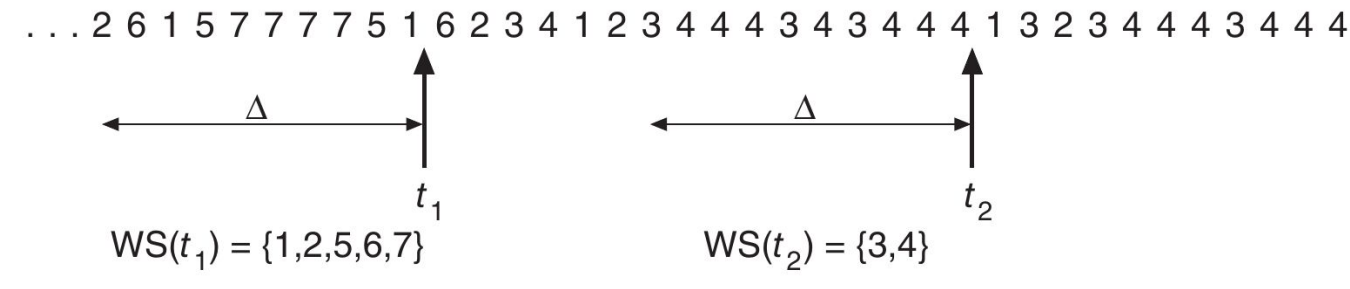
\includegraphics[width = .75\textwidth]{../res/imgs/virtual memory/working-set.png}
    \caption{Il working-set.}
    \label{fig:working-set}
\end{figure}
Definiamo ora un'altra variabile, la \textit{Working-set size}, \textbf{WSS}, che rappresenta il numero di pagine utilizzate durante la finestra $\Delta$. In particolare possiamo dire che \texttt{WSS($t_{1}$)= 5} e che \texttt{WSS($t_{2}$)= 2}. Con queste informazioni possiamo constatare che:
\vspace{-4px}
\begin{itemize}
\setlength{\itemsep}{-1px}
    \item Se $\Delta$ è molto piccolo allora non sarà possibile comprendere tutte le pagine che fanno parte della locality;
    \item Se $\Delta$ è molto grande è molto probabile che verranno comprese, oltre alla locality del processo, anche locality che non sono attive, andando quindi a sprecare memoria. 
    \item Se $\Delta \to \infty$ si andrebbero a considerare tutte le pagine del processo.
\end{itemize}
\vspace{-4px}
Chiamiamo ora con \textbf{D} $= \sum$WSS$_i$, ovvero la somma della dimensione dei working set di tutti i processi. Se D è maggiore del numero dei frames disponibili allora si è in una situazione di thrashing. Ogni sistema operativo tiene traccia di questi WSS$_i$ al fine di evitare situazioni di thrashing, di conseguenza se vede che ci si sta per avvicinare al thrashing si occupa di terminare o mettere in pausa un processo.

% 
\subsection{Frequenza dei page fault (PFF)}
Un'alternativa alla WSS è quella di andare a manipolare la frequenza dei page fault. Questo approccio, a differenza del WSS offra una soluzione meno drastica e cerca di prevenire il verificarsi del thrashing (figura \ref{fig:PFF}). In particolare, se la frequenza dei page fault è molto alta significa che ci sono diversi processi che stanno accedendo alla memoria, di conseguenza è necessario ridurre il numero di processi.
\begin{figure}[h]
    \centering
    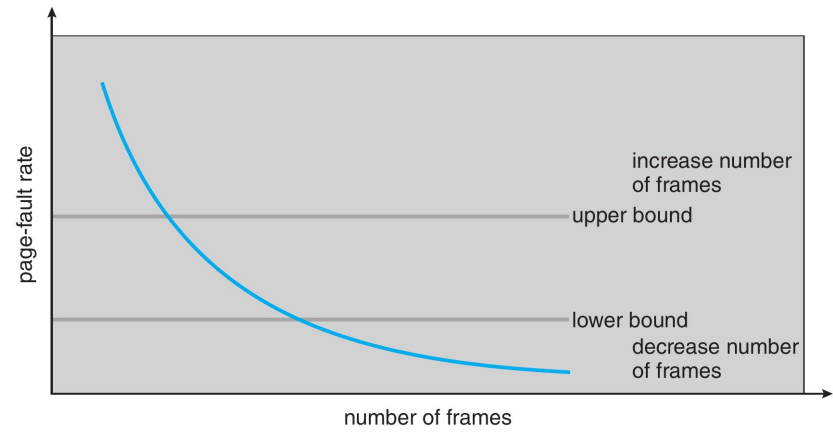
\includegraphics[width = .5\textwidth]{../res/imgs/virtual memory/PFF.png}
    \caption{Il controllo della frequenza dei page fault}
    \label{fig:PFF}
\end{figure}
Viceversa, se la frequenza di page fault è molto bassa, ciò significa che è possibile andare ad aggiungere processi in memoria.

% 
\subsubsection*{Legame tra WS e PFF}
Come è possibile vedere anche dalla figura \ref{fig:WS_vs_PFF}, esiste una relazione tra il working-set e il page fault rate. 
\begin{figure}[h]
    \centering
    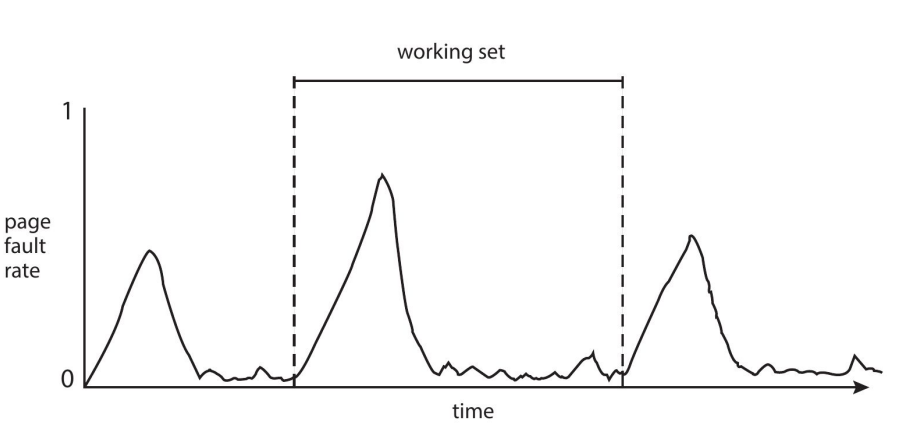
\includegraphics[width = .65\textwidth]{../res/imgs/virtual memory/WS_vs_PFF.png}
    \caption{La relazione tra working-set e page fault rate}
    \label{fig:WS_vs_PFF}
\end{figure}
Notiamo che sono presenti dei picchi di frequenza che piano piano si riducono. Questi picchi rappresentano il cambiamento di locality: quando il processo cambia da una locality ad un'altra, per un certo tempo si genereranno page fault fino a che tutti i frames necessari sono caricati in memoria.

% 
\section{Allocare la memoria del kernel}
Fino ad ora abbiamo visto la gestione della memoria in \textbf{modalità utente}. Ovviamente sono presenti anche dei modi dedicati al fine di allocare la memoria da parte del kernel del sistema operativo. Essendo infatti una parte molto importante e delicata, l'accesso in memoria non può essere rallentato a causa di altri processi: ha infatti un accesso privilegiato ed efficiente alla memoria. Sono presenti due strategie al fine di riuscire ad allocare la memoria da parte del kernel: il \textit{buddy system} e la \textit{slab allocation}.

% 
\subsection{Buddy system}
Con questo approccio la memoria è allocata da un segmento di dimensione fissata che consiste di pagine contigue (figura \ref{fig:buddy_system}). La memoria viene allocata utilizzando il \textbf{power-of-2-allocator}:
\begin{figure}[h]
    \centering
    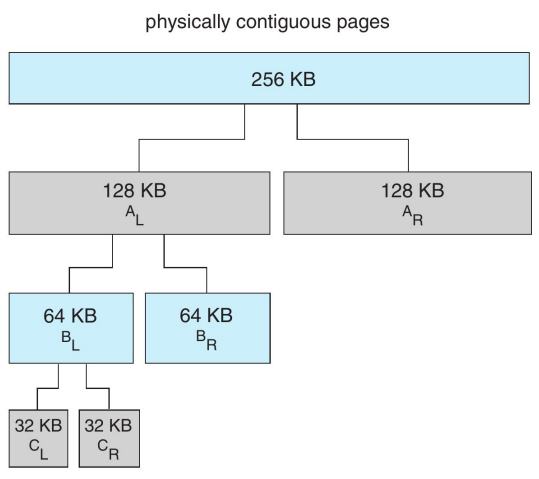
\includegraphics[width = .4\textwidth]{../res/imgs/virtual memory/buddy_system.png}
    \caption{L'approccio di allocaziony buddy system con l'allocatore \textit{power-of-2-allocator}.}
    \label{fig:buddy_system}
\end{figure}
se, per esempio, abbiamo 256KB di segmento in memoria e il kernel ne richiede 31KB, i 26KB vengono divisi per due fino a che non si arriva al blocco ideale per la richiesta effettuata dal kernel. Sa la richiesta fosse stata 33KB, si sarebbe dovuta allocare in un blocco da 64KB. Lo svantaggio sta proprio qui, dove lo spazio in memoria raramente è utilizzato ottimamente in quanto tipicamente le richieste del kernell non sono potenze di due: è il famoso fenomeno della frammentazione interna (\ref{frammentazione}).

% 
\subsection{Slab allocation}
Il secondo approccio è l'allocazione a "lastre". Questo metodo raggruppa delle pagine in memoria fisicamente contigue in \textbf{slab}; inoltre, gruppi di slabs costituiscono una \textbf{cache} (figura \ref{fig:slab_allocation}).
\begin{figure}[h]
    \centering
    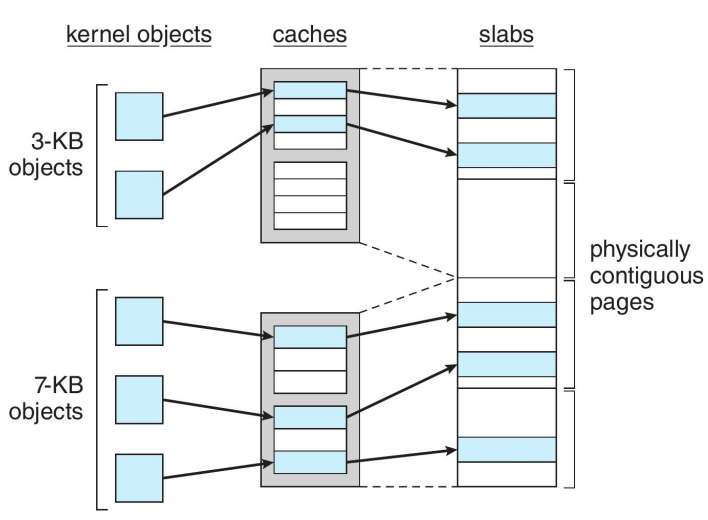
\includegraphics[width = .55\textwidth]{../res/imgs/virtual memory/slab_allocation.png}
    \caption{La slab allocation del kernel.}
    \label{fig:slab_allocation}
\end{figure}
Ad ogni struttura dati che il kernel utilizza è associata una cache. Sarà quindi presente una cache per gestire la lista dei processi (lista dei PCB \ref{PCB}), una cache per gestire la lista delle pagine e così via. Una volta che il kernel definisce le strutture che vengono usate, vengono allocate le cache volte a contenerle ed, eventualmente, ne incrementa la dimensione nel caso in cui il numero di istanze nelle strutture dati aumenti. Uno dei benefici di questa tecnica è che non si verifica la frammentazione ma comunque l'accesso rimane veloce.
